\documentclass[10pt,a4paper]{ctexart}
\usepackage[margin=2cm]{geometry}
\usepackage{graphicx}
\usepackage{hyperref}
\usepackage{amsmath}    % 提供方程环境
\usepackage{amssymb} 
\usepackage{physics}    % 简化向量、微分算子语法
\newcommand{\myspace}[1]{\par\vspace{#1\baselineskip}} %自定义空一行
\usepackage{fancyhdr}
\usepackage{wrapfig}
\usepackage{multirow}
\usepackage{booktabs} % 添加 booktabs 宏包
\usepackage{float}
\pagestyle{fancy}
\fancyhf{}  % 清除所有页眉页脚
\fancyfoot[C]{\thepage}  % 在页脚中央设置页码
\renewcommand{\headrulewidth}{0pt}  % 去掉页眉横线
\renewcommand{\footrulewidth}{0pt}  % 去掉页脚横线
% hyperref 已在上方加载一次，避免重复加载
\hypersetup{
    colorlinks=true,
    linkcolor=blue,
    filecolor=magenta,      
    urlcolor=cyan,
    pdftitle={Biprism Experiment},
    pdfpagemode=FullScreen,
    }

\usepackage{titlesec}

% 重新定义section格式
\titleformat{\section}
  {\normalfont\Large\bfseries}
  {\chinese{section}、}
  {0pt}
  {}

% 给出常用字号的自定义指令
\newcommand{\chuhao}{\fontsize{42pt}{48pt}\selectfont}
\newcommand{\xiaochu}{\fontsize{36pt}{42pt}\selectfont}
\newcommand{\xiaoer}{\fontsize{18pt}{21.6pt}\selectfont}
\newcommand{\sanhao}{\fontsize{16pt}{20pt}\selectfont}
\newcommand{\xiaosan}{\fontsize{15pt}{18pt}\selectfont}
\newcommand{\sihao}{\fontsize{14pt}{18pt}\selectfont}
\newcommand{\xiaosi}{\fontsize{12pt}{16pt}\selectfont}
\newcommand{\wuhao}{\fontsize{ 10.5pt}{12.6pt}\selectfont}

% 定义中文数字转换
\titleformat{\section}
  {\normalfont\Large\bfseries}
  {\zhnum{section}、}  % 使用\zhnum而不是\chinese
  {0pt}
  {}

% 标题设置
\title{\xiaochu\textbf{物理实验报告}}
\author{}
\date{}

\begin{document}

\vspace*{36pt} % 顶部空白

% 居中填写区域
\begin{center}
         
\includegraphics[width = 9cm]{figures/head.png} 
  
    \xiaochu\textbf{物理实验报告}
    % 预留空白区域
    \vspace{13pt}
    \vspace{13pt}
    \vspace{13pt}
    \vspace{13pt}
    
    \sanhao\textbf{实验名称：\underline{\makebox[8cm]{ 双棱镜干涉实验 }}} \\[10pt]
    \sanhao\textbf{实验桌号：\underline{\makebox[8cm]{  }}} \\[10pt]
    \sanhao\textbf{指导教师：\underline{\makebox[8cm]{ }}} \\[20pt]
    
    % 预留空白区域
    \myspace{7}
    
   \sihao\textbf{班级：\underline{\makebox[6cm]{cc98}}} \\[10pt]
    \sihao\textbf{姓名：\underline{\makebox[6cm]{Hydrofoil}}} \\[10pt]
    \sihao\textbf{学号：\underline{\makebox[6cm]{324010}}} \\[30pt]
    
    \sihao\textbf{实验日期: \underline{\makebox[0.8cm]{2026}}年 \underline{\makebox[0.4cm]{1}}月\underline{\makebox[0.4cm]{5}}日  星期\underline{\makebox[0.6cm]{一}}上午}
    
   
    \vspace{18pt}
    \sihao 浙江大学物理实验教学中心
    
\end{center}

\newpage

\section{预习报告}


    \subsection{实验综述}  

    \xiaosi （自述实验现象、实验原理和实验方法，不超过500字，5分）

    \begin{wrapfigure}{r}{0.4\textwidth}
    \centering
         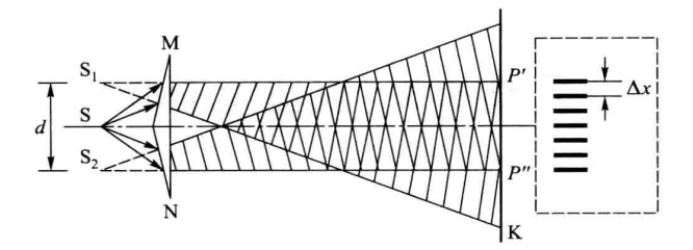
\includegraphics[width=8cm]{figures/1.png} 
    \caption{双棱镜干涉原理示意图}
    \label{fig:principle}
    \end{wrapfigure}

    \

    \subsubsection*{双棱镜干涉原理:}

    菲涅耳双棱镜实验属于分波前干涉。双棱镜由两块底面重合的直角棱镜构成，具有极小的楔角（通常 $<1^\circ$）。当单色线光源（狭缝 $S$）发出的光波入射到双棱镜上时，经过棱镜的两次折射，光束被分成两部分，分别通过棱镜的上半部和下半部。这两束光看起来像是从两个虚光源 $S_1$ 和 $S_2$ 发出的。由于 $S_1$ 和 $S_2$ 均来自同一个实际光源 $S$，它们满足相干条件（频率相同、振动方向相同、相位差恒定）。
    
    在双棱镜后方的重叠区域（干涉场）内，来自 $S_1$ 和 $S_2$ 的相干光发生干涉，形成明暗相间、等间距的平行直条纹。
    
    \subsubsection*{光波波长测定原理:}

     \begin{wrapfigure}{r}{0.4\textwidth}
    \centering
         
\includegraphics[width=8cm]{figures/图片2.png} 
    \caption{波长测定原理示意图}
    \label{fig:principle}
    \end{wrapfigure}


    在双棱镜干涉实验中，通过测量干涉条纹间距来计算光波波长。
    如图所示，设两个虚光源 $S_1$ 和 $S_2$ 之间的距离为 $d$，它们到光屏（测微目镜焦平面）的距离为 $D$。考察屏上某一点 $P$，其偏离中心的距离为 $x$。
    
    根据杨氏干涉原理，两束相干光到达点 $P$ 的光程差 $\delta$ 可近似表示为：
    \begin{align*}
        \delta \approx d \sin \theta \approx d \frac{x}{D}
    \end{align*}
    
    对于第 $k$ 级暗纹，其位置记为 $x_k$，光程差 $\delta_k$ 满足：
    \begin{align*}
        \delta_k = d \frac{x_k}{D}
    \end{align*}
    
    对于相邻的第 $k+1$ 级暗纹，其位置记为 $x_{k+1}$，光程差 $\delta_{k+1}$ 满足：
    \begin{align*}
        \delta_{k+1} = d \frac{x_{k+1}}{D}
    \end{align*}
    
    相邻两级暗纹的光程差之差应为一个波长 $\lambda$（即 $\delta_{k+1} - \delta_k = \lambda$），代入上式可得：
    \begin{align*}
        \lambda = \frac{d}{D} (x_{k+1} - x_k)
    \end{align*}
    
    令相邻条纹间距 $\Delta x = x_{k+1} - x_k$，整理即得波长测定公式：
    \begin{align*}
        \lambda = \frac{d}{D} \Delta x
    \end{align*}
    
    实验中，通过测微目镜测出 $\Delta x$，并配合二次成像法测出 $d$ 和 $D$，即可计算出待测光波的波长 $\lambda$。

    \subsubsection*{二次成像法测量虚光源间距 $d$:}

    \begin{wrapfigure}{r}{0.4\textwidth}
    \centering
         
\includegraphics[width=6cm]{figures/图片1.png} 
    \caption{二次成像法原理示意图}
    \label{fig:principle}
    \end{wrapfigure}

    由于虚光源 $S_1$ 和 $S_2$ 是不可见的，直接测量其间距 $d$ 较为困难且误差较大。本实验采用“二次成像法”（Bessel法）借助凸透镜进行间接测量。
    
    在狭缝与光屏距离 $D$ 保持不变（且 $D > 4f$，其中 $f$ 为凸透镜焦距）的情况下，移动凸透镜，可以在光屏上找到两个位置，使虚光源 $S_1, S_2$ 分别成清晰的实像。
    
    1. 当透镜靠近狭缝时，成放大的实像，测得两像间距为 $d_1$；
    2. 当透镜靠近光屏时，成缩小的实像，测得两像间距为 $d_2$。
    
    根据几何光学放大率关系，可推导出虚光源间距 $d$ 为：
    \begin{align*}
        d = \sqrt{d_1 d_2}
    \end{align*}
    
    同时，通过透镜成像公式，可利用光具座上的读数精确测量距离参数。本实验中，通过测量干涉条纹间距 $\Delta x$ 以及 $d_1, d_2$ 和 $D$，即可计算出激光波长 $\lambda$。

    \subsection{实验重点}

    \xiaosi（简述本实验的学习重点，不超过100字，3分）

    \begin{enumerate}   
        \item 掌握分波前干涉（双棱镜干涉）的基本原理；
        \item 掌握光路共轴调节技巧，特别是激光束、狭缝、双棱镜主截面的对准；
        \item 理解并运用二次成像法（Bessel法）间接测量虚光源间距 $d$；
        \item 熟练使用测微目镜精确测量细小的干涉条纹间距。
    \end{enumerate}  
    
    
    \subsection{实验难点}
    
    \xiaosi（简述本实验的实现难点，不超过100字，2分）

    \begin{enumerate}    
        \item \textbf{光路调节难}：需确保狭缝方向与双棱镜棱脊严格平行，否则干涉条纹模糊或倾斜；同时需调节系统共轴，保证光斑打在各元件中心。
        \item \textbf{干涉图样寻找}：双棱镜折射角很小，干涉区域窄，需细致调节前后距离和横向位置才能在目镜中观察到清晰条纹。
        \item \textbf{微弱信号观测}：二次成像中，缩小像的光强较弱且间距小，容易被背景杂散光干扰，需仔细辨别。
        \item \textbf{空程差消除}：使用测微目镜测量条纹间距时，必须单向旋转鼓轮以消除螺距空程差。
    \end{enumerate}  


\section{原始数据}

   
    \xiaosi （将有老师签名的“自备数据记录草稿纸”的扫描或手机拍摄图粘贴在下方，20分）

    \begin{figure}[htbp]
        \centering
                
\includegraphics[width=14cm]{figures/实验数据.jpg} 
        \label{fig:raw_data}
    \end{figure}

\newpage
    
\section{结果与分析}

    \subsection{数据处理与结果}
    \xiaosi （列出数据表格、选择数据处理方法、给定测量或计算结果，30分）
    
    \
    
    \textbf{1. 实验参数记录：}
    
    毛玻璃屏位置 $v_0 = 146.0 \text{ cm}$，狭缝位置 $15.01 \text{ cm}$，双棱镜位置 $35.11 \text{ cm}$。
    
    \textbf{2. 二次成像法测量虚光源间距 $d$ 及距离 $D$：}

    利用凸透镜两次成像测量虚光源的放大像间距 $d_1$ 和缩小像间距 $d_2$。

    \begin{table}[H]
    \centering 
    \caption{二次成像法测量数据表}
    \label{tab:bessel_method} 
    \begin{tabular}{cccccc}
        \toprule
        \multirow{2}{*}{次数} & \multicolumn{2}{c}{透镜位置 (cm)} & 放大像间距 & 缩小像间距 & 虚光源间距 \\
        \cmidrule(lr){2-3} 
        & $v_{O1}$ (放大) & $v_{O2}$ (缩小) & $d_1$ (mm) & $d_2$ (mm) & $d=\sqrt{d_1 d_2}$ (mm) \\ 
        \midrule
        1 & 60.47 & 99.08 & 5.564 & 1.689 & 3.066 \\
        2 & 60.43 & 99.36 & 5.531 & 1.649 & 3.020 \\
        3 & 60.57 & 99.19 & 5.536 & 1.665 & 3.036 \\
        4 & 60.64 & 99.18 & 5.574 & 1.669 & 3.050 \\
        5 & 60.55 & 99.34 & 5.530 & 1.638 & 3.010 \\
        6 & 60.70 & 99.26 & 5.557 & 1.609 & 2.990 \\
        \bottomrule
    \end{tabular}
    \end{table}

    实验时的物屏间距固定为 $D = 132.45 \text{ cm} = 1324.5 \text{ mm}$ 。
    
    计算 $d$ 的平均值及其不确定度：
    \begin{align*}
        \bar{d} &= \frac{1}{6}\sum_{i=1}^6 d_i = 3.029 \text{ mm} \\
        u_A(d) &= \sqrt{\frac{\sum(d_i - \bar{d})^2}{6(6-1)}} \approx 0.012 \text{ mm}
    \end{align*}

    \myspace{1}

    \textbf{3. 干涉条纹间距 $\Delta x$ 测量：}
    
    利用测微目镜测量 10 个条纹的宽度，以提高测量精度。测量第 $i$ 条与第 $i+10$ 条暗纹的位置 $S_i$ 和 $S_{i+10}$。

    \begin{table}[H]
    \centering 
    \caption{干涉条纹间距测量数据表 (单位：mm)}
    \label{tab:fringes} 
    \begin{tabular}{cccc}
        \toprule
        编号 & 起始位置 $S_i$ (mm) & 终止位置 $S_{i+10}$ (mm) & $10\Delta x = S_{i+10} - S_i$ (mm) \\
        \midrule
        1 & $S_1 = 0.000$ & $S_{11} = 2.790$ & 2.790 \\
        2 & $S_2 = 0.284$ & $S_{12} = 3.060$ & 2.776 \\
        3 & $S_3 = 0.547$ & $S_{13} = 3.344$ & 2.797 \\
        4 & $S_4 = 0.847$ & $S_{14} = 3.600$ & 2.753 \\
        5 & $S_5 = 1.119$ & $S_{15} = 3.906$ & 2.787 \\
        6 & $S_6 = 1.392$ & $S_{16} = 4.169$ & 2.777 \\
        \bottomrule
    \end{tabular}
    \end{table}

    计算 $10\Delta x$ 的平均值：
    \begin{align*}
        \overline{10\Delta x} &= \frac{2.790 + 2.776 + 2.797 + 2.753 + 2.787 + 2.777}{6} = 2.780 \text{ mm} \\
        \therefore \overline{\Delta x} &= 0.2780 \text{ mm}
    \end{align*}

    计算 $y = 10\Delta x$ 的A类不确定度：
    \begin{align*}
        u_A(y) = \sqrt{\frac{\sum(y_i - \bar{y})^2}{6(5)}} \approx 0.0063 \text{ mm}
    \end{align*}

    \myspace{1}

    \textbf{4. 波长 $\lambda$ 计算及不确定度分析：}

    根据公式 $\lambda = \frac{d \cdot \Delta x}{D} = \frac{d \cdot y}{10 D}$，代入平均值：
    \begin{align*}
        \bar{\lambda} = \frac{3.029 \text{ mm} \times 2.780 \text{ mm}}{10 \times 1324.5 \text{ mm}} \approx 6.357 \times 10^{-4} \text{ mm} = 635.7 \text{ nm}
    \end{align*}

    \textbf{不确定度合成：}
    
    1. \textbf{仪器误差 (B类不确定度)}：
       \begin{itemize}
           \item 读数显微镜：$\Delta_{micro} = 0.004 \text{ mm}$，则 $u_B(y) = 0.004/\sqrt{3} \approx 0.0023 \text{ mm}$。
           \item 光具座直尺：$\Delta_{rule} = 0.2 \text{ mm}$ (估读)，用于 $D$ 的测量。$u_B(D) = 0.2/\sqrt{3} \approx 0.12 \text{ mm}$。
       \end{itemize}

    2. \textbf{合成各分量不确定度}：
       \begin{align*}
           u(y) &= \sqrt{u_A(y)^2 + u_B(y)^2} = \sqrt{0.0063^2 + 0.0023^2} \approx 0.0067 \text{ mm} \\
           u(d) &\approx u_A(d) = 0.012 \text{ mm} \quad (\text{忽略} d_1, d_2 \text{测量的B类分量，以A类为主}) \\
           u(D) &\approx 0.2 \text{ mm} \quad (\text{单次测量，主要为B类})
       \end{align*}

    3. \textbf{波长合成相对不确定度}：
       依据公式 $\ln \lambda = \ln d + \ln y - \ln(10D)$，有：
       \begin{align*}
           \frac{u(\lambda)}{\lambda} &= \sqrt{\left(\frac{u(d)}{d}\right)^2 + \left(\frac{u(y)}{y}\right)^2 + \left(\frac{u(D)}{D}\right)^2} \\
           &= \sqrt{\left(\frac{0.012}{3.029}\right)^2 + \left(\frac{0.0067}{2.780}\right)^2 + \left(\frac{0.2}{1324.5}\right)^2} \\
           &= \sqrt{(0.39\%)^2 + (0.24\%)^2 + (0.015\%)^2} \approx 0.46\%
       \end{align*}
       
       \textbf{最终结果：}
       \begin{align*}
           u(\lambda) &= 635.7 \times 0.46\% \approx 3 \text{ nm} \\
           \therefore \lambda &= (636 \pm 3) \text{ nm}
       \end{align*}

    \subsection{误差分析}
    \xiaosi （运用测量误差、相对误差、不确定度等分析实验结果，20分）
    
    \begin{enumerate}
        \item \textbf{视差与读数误差}：使用读数显微镜测量 $d_1, d_2$ 及条纹间距时，十字叉丝与像面的聚焦可能存在轻微视差，且人眼判断叉丝是否对准条纹中心（或明暗边界）存在主观误差。
        \item \textbf{空程差}：读数显微镜的螺杆存在空程，如果在测量过程中往复转动鼓轮，会引入显著的系统误差。实验中应严格保持单向旋转。
        \item \textbf{光具座水平与共轴误差}：若导轨不水平或光路非严格共轴，会导致透镜移动过程中光轴偏离，使得测得的 $D, d_1, d_2$ 值不准确。
        \item \textbf{条纹倾斜}：若狭缝与双棱镜棱脊不严格平行，干涉条纹会发生倾斜。此时垂直于条纹移动测微目镜测得的间距 $\Delta x'$ 会大于实际间距 $\Delta x$，导致波长计算值偏大。
        \item \textbf{小间距测量误差}：$d_2$ 通常很小（约 1.6 mm），相对测量误差较大，对 $d$ 的合成不确定度贡献显著。
    \end{enumerate}

    \subsection{实验探讨}
    \xiaosi （对实验内容、现象和过程的小结，不超过100字，10分）

    \myspace{1}

    本次实验通过双棱镜干涉测定了激光波长，加深了对分波前干涉原理的理解。掌握了利用“二次成像法”测量微小虚光源间距的技巧。实验中发现，光路的共轴调节和狭缝方向的精细校准是获得清晰、平直干涉条纹的关键，直接影响测量精度。       
    
    \section{思考题}

    \xiaosi （解答教材或讲义或老师布置的思考题，10分）

    \subsubsection*{1. 为减小测量误差，应该如何设置狭缝到屏的距离 $D$，狭缝到双棱镜的距离？}


    \begin{enumerate}
        \item \textbf{狭缝到屏的距离 $D$}：应适当\textbf{增大} $D$。根据 $\Delta x = \frac{D}{d}\lambda$，增大 $D$ 会使条纹间距 $\Delta x$ 变宽，从而降低测微目镜读数的相对误差。但 $D$ 也不宜过大，否则条纹亮度会降低，且需满足 $D > 4f$ 以确保能进行二次成像。
        \item \textbf{狭缝到双棱镜的距离}：应适当\textbf{减小}该距离。减小狭缝到双棱镜的距离会减小虚光源间距 $d$（因为 $d \approx 2(n-1)\alpha l_1$，其中 $l_1$ 是狭缝到棱镜距离）。$d$ 减小同样会使条纹间距 $\Delta x$ 增大，便于测量。
    \end{enumerate}

    \subsubsection*{2. 测量时如果条纹有倾斜，对测量结果有何影响？}

    \textbf{答：}
    如果条纹倾斜（即狭缝与双棱镜棱脊不平行），而测微目镜的移动方向是水平的（垂直于光轴），那么测量的是斜向截割条纹的距离。
    
    设条纹倾角为 $\theta$，实际条纹间距为 $\Delta x$，测量值为 $\Delta x_{meas}$，则有关系 $\Delta x_{meas} = \frac{\Delta x}{\cos \theta}$。
    
    由于 $\cos \theta < 1$（当 $\theta \neq 0$），所以 $\Delta x_{meas} > \Delta x$。这将导致代入公式 $\lambda = \frac{d \Delta x}{D}$ 计算出的波长值\textbf{偏大}。因此实验中必须调节狭缝旋转旋钮，使条纹严格竖直。

\newpage

\sihao\textbf{注意事项：}
\xiaosi
\begin{enumerate}
    \item  用 PDF 格式上传“实验报告”，文件名：学生姓名+学号+实验名称+周次。
    \item  “实验报告”必须递交在“学在浙大”的本课程的对应实验项目的“作业”模块内。
    \item  “实验报告”成绩必须在“浙江大学物理实验教学中心网站”-“选课系统”内查询。
    \item 教学评价必须在“浙江大学物理实验教学中心网站”-“选课系统”内进行，学生必须进行教学评价，才能看到实验报告成绩，教学评价必须在本次实验结束后 3 天内进行。
\end{enumerate}

\vspace{1cm}
\xiaosi\centering \textbf{浙江大学物理实验教学中心制}

\end{document}